%----------------------------------------------------------------------------
\section{Adatbiztonság}
{\footnotesize Fizikai, ügyviteli és algoritmusos adatvédelem, az informatikai biztonság szabályozása. Kriptográfiai alapfogalmak. Klasszikus titkosító módszerek. Digitális aláírás, a DSA protokoll.}
%----------------------------------------------------------------------------
\subsection{Fizikai, ügyviteli és algoritmusos adatvédelem, az informatikai biztonság szabályozása.}
\begin{definition}[Adatvédelem]
	azon fizikai, ügyviteli és algoritmikus eszközök együttes felhasználását értjük, amelyek segítségével a véletlen adatvesztések és szándékos adatrongálódások és információ kiszivárogtatások megelőzhetők, vagy jelentős mértékben megnehezíthetők
\end{definition}
\paragraph{Fizikai adatvédelem} két lényegi dolgot takar: Egyrészt biztosítani kell az optimális, de legalább a még elfogadható \textbf{üzemi körülményeket} (hőmérséklet, páratartalom, por, tartalék alkatrészek stb.), másrészt pedig a szükséges \textbf{vagyonvédelmi intézkedésekről} sem szabad megfeledkezni. Például: Villamos hálózat helyes kialakítása; Szünetmentes tápegységek használata; Megfelelő szerverterem kialakítása(klimatizálás, füstérzékelés, árnyékolás,\dots); Megfelelő adattároló eszközfajták használata; Betörésvédelem.

\paragraph{Ügyviteli adatvédelem} a folyamatok szabályozásának, a szabályzatoknak a kialakítása és védelme. A fizikai adatvédelem önmagában ugyanis nem elegendő. Példa: hiába zárjuk be a szerverszoba ajtaját, ha a portás beengedi azt, aki egy szerszámos táskával érkezvén arról tájékoztatja, hogy ’zsírozni kell a switcheket’ (social hacking/engineering). Tehát szükséges \textbf{pontosan szabályozni}, hogy \textbf{ki}, \text{mikor}, \textbf{mit} és \textbf{hogyan} tehet meg, illetve nem tehet meg. Szükség van \textbf{informatikai biztonsági szabályzatra} is, amely mindezt egységes módon áttekinti. Megfelelő felhasználó menedzselési rendet kell kialakítani, hogy a felhasználók, hozzáférési jogosultságaik, munkájukból adódó szerepköreik kezelése összhangba hozható legyen. Példák: Feladat- és jogkörök szétválasztása; Hozzáférések és tevékenységek regisztrálása; Személyazonosítás; Hatáskörök és felelősségek szétválasztása vagy átlapolása.

\paragraph{Algoritmikus adatvédelem} feladata olyan programok és eljárások alkalmazása, amelyek segítik az előző két terület feladatait és létrehozzák azokat a számítógépes védelmi funkciókat, amik ezen a területen meggátolják az adatokhoz való illetéktelen hozzáférést és módosítást. Példák: Hálózati azonosítás; \textbf{Titkosítás}; Behatolásvédelem; Automatikus adatmentés; Többforrásos adattárolás.

\paragraph{Az informatikai biztonsági szabályrendszer szükségessége:} (1) az adatok egyre inkább elektronikus formában jelennek meg; (2) a Szervezetek informatika nélkül működésképtelenek; (3) az informatikai függőség egyre nagyobb; (4) ugyanakkor a fenyegetettség is egyre növekszik; (5) az üzletfolytonossághoz kritikus fontosságú; (6) a kárpotenciál és a kockázati tényezők szervezetenként eltérőek lehetnek!

\subsubsection{Biztonsági célok}
Alapkövetelmények, amelyek teljesülése az üzemszerű használhatóság előfeltétele:
\begin{enumerate}
	\item rendelkezésre állás (elérhetőség az arra jogosultak számára)
	\item sértetlenség (valódiság)
	\item bizalmasság (jellegtől függően)
	\item nyomon követhetőség, hitelesség
	\item Biztosítékok (az információs rendszer teljességére nézve)
\end{enumerate}
Ez alapján úgy lehet meghatározni az Informatikai Biztonság fogalmát, hogy az akkor áll fenn, ha az információs rendszer védelme az alapkövetelmények szempontjából
\begin{itemize}
	\item \textbf{zárt:} minden fontos fenyegetést figyelembe vesz
	\item \textbf{teljes körű:} a rendszer összes elemére kiterjedő
	\item \textbf{folyamatos:} megszakítás nélküli, az időben változó körülmények ellenére is
	\item \textbf{kockázatarányos:} a feltehető kárérték és a kár valószínűségének szorzata nem haladhat meg egy előre rögzített küszöböt, amely egy üzleti döntés.
\end{itemize}

\subsection{Kriptográfiai alapfogalmak.}
\begin{center}
	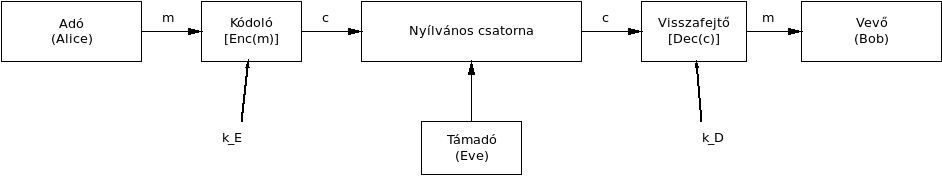
\includegraphics[width=0.7\linewidth]{fig/14-Crypto_scheme}
\end{center}
\begin{definition}[titkostási rendszer]
	A $(\mathcal{P}, \mathcal{C}, \mathcal{K},Enc,Dec,Key)$ hatost titkosítási rendszernek (sémának) nevezzük, ahol:
	\begin{itemize}[nosep]
		\item $\mathcal{P}, \mathcal{C}, \mathcal{K}$ a nyílt és titkos üzenetek, valamint lehetséges kulcsok véges, nemüres halmaza ($1<|\mathcal{P}|,|\mathcal{C}|,|\mathcal{K}| < \infty$).
		\item $Enc:\; \mathcal{K}\times\mathcal{P} \to c\;$ egy titkosító függvény ($c \in \mathcal{C}$: titkosított üzenet)
		\item $Dec:\; \mathcal{K}\times\mathcal{C} \to m\;$ egy visszafejtő függvény ($m \in \mathcal{P}$: nyílt üzenet)
		\item $Key \subseteq \mathcal{K}\times\mathcal{K}$ kulcspárok halmaza
	\end{itemize}
\end{definition}
\begin{definition}[Korrekt visszafejtés]
	A titkosító rendszer korrekt visszafejtést biztosít, ha minden $(k_E,k_D)\in\mathcal{K},\; m\in\mathcal{P}$ esetén
	$$Dec(k_D,Enc(k_E,m)) = m$$
\end{definition}
\begin{note}~\\
	\begin{itemize}[nosep]
		\item $(k_E,k_D)$ titkosító-visszafejtő kulcspár
		\item $c = Enc(k_E,m)$
		\item definíció alapján, rögzített $(k_E,k_D)$ esetén az $Enc_{k_E}(m) = Enc(k_E,m)$ függvény injektív, azaz:
		$$Enc_{k_E}(m_1) = Enc_{k_E}(m_2) \Leftrightarrow m_1 = m_2$$
	\end{itemize}
\end{note}
\begin{definition}[Teljes titkosítási rendszer]
	A titkosítási rendszert teljesnek nevezzük, ha minden $(k_E,k_D)$ esetén az $Enc_{k_E}(m)$ függvény szürjektív, azaz minden $c\in\mathcal{C}$ titkos üzenet esetén létezik $m\in\mathcal{P}$ nyílt üzenet, amelyikre $Enc_{k_E}(m) = c$. Ebben az esetben $|\mathcal{P}| = |\mathcal{C}|$
\end{definition}
Természetes elvárás egy titkosítási rendszerrel szemben, hogy ha vannak $k_{E1} \neq k_{E2}$ kulcsok, akkor $Enc_{k_{E1}}(m) \neq Enc_{k_{E2}(m)}$. Továbbá ha $(k_E,k_{D1}), (k_E,k_{D2})\in Key$, akkor $k_{D1} = k_{D2}$.
\begin{definition}[Teljes kulcstér]
	Legyen $|\mathcal{P}| = |\mathcal{C}|$ . A kulcsteret teljesnek nevezzük, ha minden $f:\;\mathcal{P} \to \mathcal{C}$ bijektív leképezéshez létezik $k_E \in \mathcal{K}$, amelyikre $Enc_{k_E} = f$.
\end{definition}
\begin{description}[nosep]
	\item[Kriptográfia] A kulcs alapú titkosítási technikák tudománya
	\item[Kriptanalízis] A kulcs alapú titkosítási technikák feltörésének, támadásának tudománya
	\item[Kriptológia] Kriptográfia + Kriptanalízis
	\item[Nyílt szöveg (plain text)] Az eredeti, mindenki által értelmezhető információ
	\item[Titkosított szöveg (ciphertext)] A titkosított információ
	\item[Titkosítás (encryption)] Eljárás, mely során az információt a birtokosa titkossá nyilvánít.
	\item[Visszafejtés (decryption)] A titkosított információból az eredeti visszaállítása.
	\item[Rejtjelezés] Adott módszer a nyílt szöveg kódolására (és visszafejtésére)
	\item[Kulcs (key)] Az az információ, amelynek segítségével a rejtjelezés történik. Két típus: nyilvános és titkos kulcs.
	\item[Szimmetrikus titkos. rendszer] Ha van $(k_E,k_D)$ kulcspárunk, $k_E$ nyílvános kulcs megegyezik a $k_D$ titkos kulccsal vagy $k_D$ polinomiális időben kiszámolható $k_E$-ből.
	\item[Aszimmetrikus titkos. rendszer] A tetszőlegesen választott $k_E$ és $k_D$ kulcspárok annyira különböznek, hogy nem létezik polinomiális időbonyolultságú algoritmus, mely $k_E$-ből kiszámolja $k_D$-t
\end{description}

\subsection{Klasszikus titkosító módszerek.}
A számítógép megjelenése előtt (before computers, BC) használt rendszereket, történelmi vagy klasszikus titkosítási rendszereknek nevezzük. Nem egyértelműen definiált, de nagyjából a számítógéppel könnyen támadható rendszereket nevezzük így. Jellemzően élő nyelvi szöveg titkosítására használták. Főbb típusai:
\begin{easylist}[enumerate]
	# Helyettesítéses titk. rendszerek: Az üzenet egy betűjét más betűre vagy szimbólumra cseréli
	## monoalfabetikus: a csere transzformációja változatlan
	## polialfabetikus: az egymás után következő betűket más-más transzformációval titkosítjuk
	# Permutációs titk. rendszerek: az üzenet betűit más sorrendben írjuk fel (mint egy anagramma, de a titkos szöveg nem feltétlenül értelmes)
\end{easylist}
\paragraph{Betűk kicserélése absztrakt szimbólumokra} Helyettesítéses, monoalfabetikus
\paragraph{Caesar--titkosítás} Monoalfabetikus, helyettesítéses.\\
$Enc_k(m) = k+m (mod\; 26)$\\
$Dec_k(c) = c-k (mod\; 26)$
\paragraph{Affin titkosítás} Monoalfabetikus\\
$k_E = (\alpha,\beta)\; k_D = (\alpha^{-1},\beta)\quad lnko(\alpha,26) = 1$\\
$Enc = \alpha \cdot m + \beta (mod\; 26)$\\
$Dec = \alpha^{-1} \cdot (c - \beta) (mod\; 26)$
\paragraph{Vigènre-titkosítás} polialfabetikus, a kulcs valamilyen karaktersorozat. A Vernam--rejtjelező (OTP) hasonló hozzá, azonban az kulcs hossza megegyezik az üzenettel. Bináris esetben a Vernam--rejtjelező az üzeneten és a kulcson bitenkénti XOR műveletet végrehajtva állítja elő a titkos üzenetet.\\
$c[i] = m[i] + k_E[i\; mod\; n] (mod\; 26)$\\
$m[i]= c[i]- k_E[i\; mod\; n] (mod\; 26)$

\paragraph{Enigma} Polialfabetikus. Elektromechanikus rejtjelező, ahol a kulcsot a gépben található tárcsák kezdőpozíciója jelentette.

\subsection{Modern titkosítási rendszerek}
\subsubsection{Folyamtitkosítás}
Bitsorozat titkosítása bitenként. Legegyszerűbb módszer a One-Time-Pad titkosítás, ahol titkosított bitsorozat, az eredeti sorozat egy álvéletlen bitsorozattal történő XOR művelet eredménye $c[i] = m[i]XORk[i]$. Shannon bebizonyította, hogy egy teljesen véletlen kulcsfolyam esetén a titkos üzenet elméletileg feltörhetetlen. Tehát ennek a titkosításnak az erőssége az álvéletlenszám-generátor erősségén múlik. Alkalmazásakor a mesterkulcsot a kulcsgenerátor kezdeti állapota jelenti. A kulcsfolyam-generálásnak több variánsa is létezik:
\paragraph{Lineárisan visszacsatolt léptető regiszter -- LFSR}
A kulcsfolyam $l$ bitjein egy $a = (a_0,a_1,\dots,a_{l-1})$ értékkel bitenkénti ÉS műveletet hajtunk végre, majd a részeredményen XOR műveletet hajtunk végre. Így kapjuk meg a $k_i$ kulcsot:
$$ k_i = a_{l-1}k_{i-1}\oplus a_{l-2}k_{i-2}\oplus\dots\oplus a_{0}k_{i-l}$$
\begin{center}
	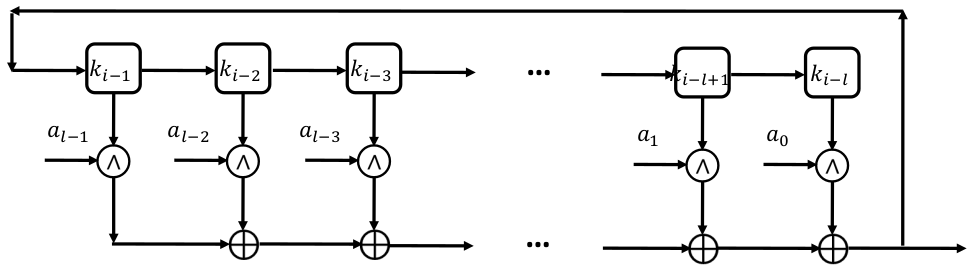
\includegraphics[width=0.7\linewidth]{fig/14-LFSR}
\end{center}
Az $a_i$ és kezdeti $k_i$ értékei adják a generátor kezdeti állapotát. Fontos, hogy ezeket az értékeket jól válasszuk meg, mert ezen múlik az álvéletlen sorozat minősége. Ez leginkább két dolgot takar: sorozat eloszlása (fontos, hogy egyenletes legyen) és a periódus hossza (minél hosszabb annál jobb).
\paragraph{Lineárisan rekurzív sorozat -- LSR}
Az LFSR általánosítása. C/C++ rand() függvénye implementálja.\\
$a = 31835, b = 1906, k_0 = 41$\\
$k_i = a \dots k_{i-1} + b (mod 2^{15})$\\
periódusa $2^{15}$
\paragraph{Blum--Blum--Shub generátor -- BBS}
$p, q$ nem közeli nagy prímek: $m = p\times q$ és $a_0$ úgy választjuk, hogy $lnko(a_0,m)=1$.\\
$a_i = a_{i-1}^2 \;(mod\; n)$
$k_i = a_i(mod 2)$ vagy például $a_i$ paritása.\\
A következő $a_i$ az előzőekből exponenciális időben számolható ki. Periódusa kb. $p\cdot q$, ha $lnko(p-1,q-1)$ kicsi, ezért kell, hogy p és q ne legyenek egymáshoz közel.
\paragraph{RC4}
\begin{multicols}{2}
Egy S kezdeti tömb feltöltése és összekeverése után a következő bitet az  %\ref{fig:14-rc4}~
ábrán látható módon kapjuk meg, (i = (i + 1) mod 256 j = j + S i mod 256).
Felhasználja az SSL/TLS, és a WEP protokoll.
\begin{center}
	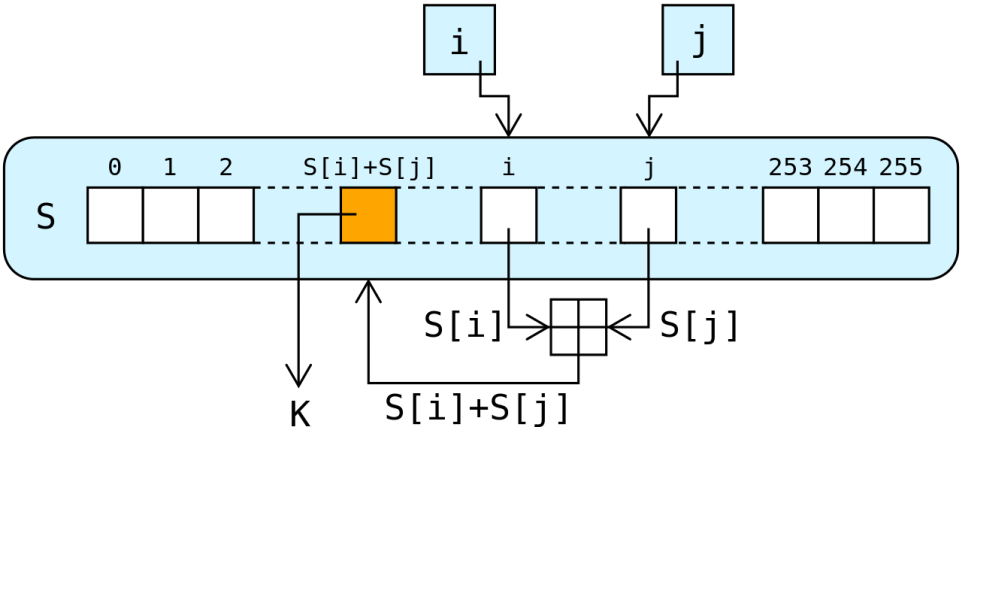
\includegraphics[width=\linewidth]{fig/14-RC4}
%	\caption{A következő elem (K) meghatározása az S tömbből. Minden kiolvasás előtt S[i] és S[j] értéket felcseréljük a tömbben}
%	\label{fig:14-rc4}
\end{center}
\end{multicols}

\subsubsection{DES}
\begin{multicols}{2}
\begin{easylist}[itemize]
# 1975-ben jelent meg, a LUCIFER titkosítási rendszer egyik változata.
# Ma már nem létezik szabványként, mert feltörték, helyette a Triple DES-t ajánlott használni. 
# Szimmetrikus, blokktitkosítási rendszer, a blokk mérete 64 bit. Ha ennél nagyobb méretű üzenetet kell titkosítani, akkor azt fel kell tördelni valamilyen blokktitkosítási módszerrel.
# Matematikai alapja a Fiestel struktúra.
# A Kulcs 64 bites, amelyből 56 bit random és 8 a random bitek alapján meghatározott. 
# S-BOX-ok használata a titkosítás és a visszafejtés során.
# 16 körből áll az algoritmus, ezért 16 körkulcs kerül legenerálásra az eredeti kulcsból. Visszafejtéskor a körkulcsokat fordított sorrendben kell alkalmazni.
# Jellemzők:
## az S-BOX-okat kivéve minden lépése az algoritmusnak lineáris
## az S-BOX-ok eredete nem ismert, de a feltételeknek megfelelnek.
## nagy problémája a kis kulcstér, ezért kell inkább TDES-t alkalmazni ma már.
\end{easylist}
\end{multicols}
\begin{figure}[h]
	\centering
	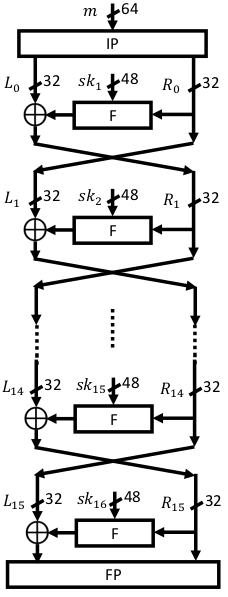
\includegraphics[width=0.2\linewidth]{fig/14-DES_Feistel_net}
	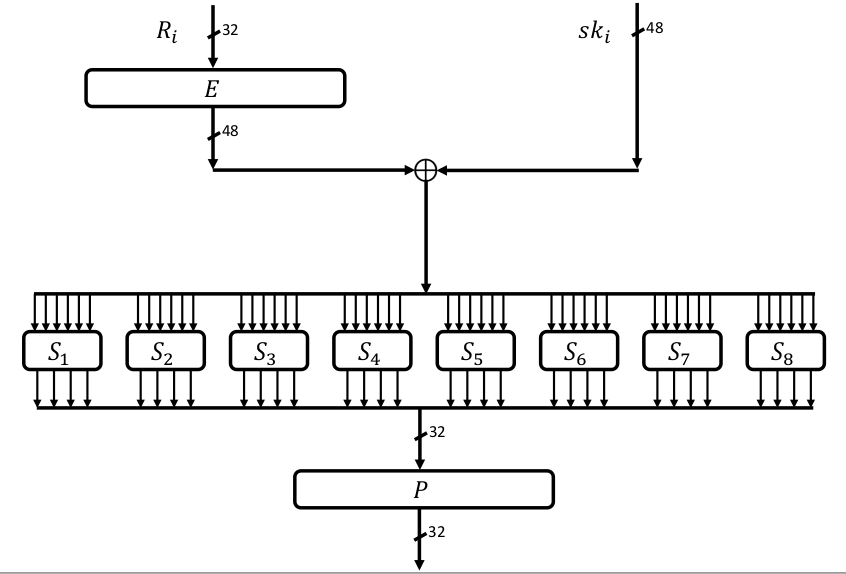
\includegraphics[width=0.7\linewidth]{fig/14-DES_Feistel_func}
	\caption{A feistel-háló és a feistel függvény (F - Feistel függvény; IP,FP - egymással ellentétes permutációk; E - kiterjesztő függvény; S - S-boxok; P - permutáció;sk - a mesterkulcsból képzett 16 részkulcs)}
	\label{fig:14-desfeistelnet}
\end{figure}

\subsubsection{AES}
\begin{multicols}{2}
\begin{easylist}[itemize]
# Szimmetrikus, blokktitkosítási rendszer. Kifejlesztői: RIJNDAEL (Vincent Rijmen, Joan Daemen).
# A (T)DES-nél hatékonyabb titkosításra képes, mivel matematikai alapja nem Fiestel struktúra, itt a bitek nem csak keverednek, de meg is változnak!
# 128, 192, 256 bites blokkhossz és kulcshossz kezelésére képes bármilyen kombinációban.
# Bonyolult matematikai háttere van, a bájtokat {0,1} együtthatós polinomként kezeli.
# Tervezésekor fontos volt az ismert támadásokkal szembeni védelem, a gyorsaság és tömör kódolhatóság
# A belső algoritmus ciklusainak száma a blokkhossz és a kulcshossz függvényében lehet 10, 12, 14
# Visszafejtésnél az összes transzformáció inverzét kell végrehajtani.
\end{easylist}
Működése 3 fő részből és 4 műveletből áll:
\begin{easylist}[enumerate]
# Előkészítés:
## AddRoundKey
# Ismételt rész:
## SubBytes
## ShiftRows
## MixColumns
## AddRoundKey
# Utófeldolgozás:
## SubBytes
## ShiftRows
## AddRoundKey
\end{easylist}
\begin{description}[nosep]
	\item[AddRoundKey] XOR művelet az állapotmátrix és a megfelelő sorszámú kulcs között
	\item[SubBytes] speciális S-boxokat használ, mely egy nemlineáris helyettesítési kódolást valósít meg
	\item[ShiftRows] a sorokat ciklikusan eltolják. Az 1. sor 0, a 2. sor 1,\dots, 4. sor 3 hellyel
	\item[MixColumns] oszloponként egy lineáris transzformáció:
	$\begin{matrix}
	2 & 3 & 1 & 1\\
	1 & 2 & 3 & 1\\
	1 & 1 & 2 & 3\\
	3 & 1 & 1 & 2
	\end{matrix}$
\end{description}
\end{multicols}

\subsubsection{RSA}
\begin{easylist}[itemize]
# Feltalálói: Ron Rivest, Adi Shamir, Leonard Adleman, 1977-ben.
# Az első aszimmetrikus, PKI-t használó kriptográfiai rendszer. (NEM BLOKKTITKOSÍTÓ RENDSZER)
# A kommunikációban résztvevő mindkét félnek rendelkeznie kell egy Publikus és egy Titkos kulccsal (PK; SK), amelyeket a kommunikáció titkosságának biztosítása érdekében felhasználnak.
# Kulcsgeneráló algoritmus, PK=(n,e) és SK=(n,d)
## Véletlenül választunk két nagy prímet: p,q
## Kiszámoljuk: n=p*q
## Kiszámoljuk: \textphi(n)=(p-1)*(q-1)
## Választunk véletlen egy e-t, hogy 1 < e < \textphi(n) és (e,\textphi(n)) = 1
## Kiszámítjuk d-t, hogy 1 < d < \textphi(n) és e*d= 1 (mod \textphi(n))
# A PK és SK ismeretében a titkosító algoritmus: 	c = ENC\textsubscript{PK}(m) = m\textsuperscript{e} (mod n)
# A PK és SK ismeretében a visszafejtő algoritmus: 	m = DEC\textsubscript{SK}(c) = c\textsuperscript{d} (mod n)
# Az RSA feltörésének nehézségét a prím-faktorizáció nehézsége adja:  \{c,n,e\} $\leftarrow$ \{m\}  nehéz!
# p és q választásánál fontos, hogy hosszuk bitekben hasonló legyen, viszont ne legyenek túl közeliek
# e választásánál, annál jobb minél kisebb, általában 65537 szokott lenni.
\end{easylist}

\subsection{Digitális aláírás, a DSA protokoll.}
A digitális aláírás lényege:
\begin{easylist}[enumerate]
# Letagadhatatlanság --- alkalmas az aláíró azonosítására 
# Hitelesítés --- más nem tudja létrehozni 
# Hamisíthatatlanság --- akár az aláírás, akár a dokumentum módosul, észrevehető.
\end{easylist}
A letagadhatatlanság és harmadik fél számára is elfogadható hitelesítés
alapvetően kétféle megoldással lehetséges:
\begin{easylist}[itemize]
# megbízható harmadik féllel (Trusted Third Party, TTP) (szigorúan véve nem DS)
# közvetlen digitális aláírás (nyilvános kulcsú titkosítással)
\end{easylist}
Digitális aláírás fajtái:
\begin{easylist}[itemize]
# RSA alapú --- Az aláíró a titkos kulcsával titkosítja az üzenetét vagy annak kivonatát. A hitelességet az adja, hogy egyedül az aláíró nyilvános kulcsa tudja visszafejteni a dokumentumot (vagy a kivonatot). Hátrányai:
## nem megbízható --> egzisztenciális hamisítás: egy tetszőleges s értéket választva előállíthatjuk az $ m \equiv s^e (n) $ üzenetet.
## alakíthatóság --> $(m_1,s_{m_1}),(m_2,s_{m_2})$ létező aláírásokból előállítható az $(m_1m_2,s_{m_1}s_{m_2})$ új aláírás
## Ezek a hátrányok nem jelentkeznek, ha az üzenet helyett annak kivonatát írjuk alá (hash-and-sign):\\
$S_m\equiv Hash(m)^d (n) \Rightarrow (m,S_m)$\\
ellenőrzés: $Hash(m) \equiv S_m^d (n)$
# ElGamal alapú --- Hátránya, hogy az aláírás kétszer akkora, mint a dokumentum
# DSA protokoll --- Digital Signature Algorithm. A digitális aláírás szabvány (DSS) felhasználja.
\end{easylist}

\subsubsection{DSA}
\begin{multicols}{2}
Kulcsgenerálás:
\begin{enumerate}[nosep]
	\item $p, q$ olyan prímek, hogy $q|p-1$ (p-1 q többszöröse)
	\item meghatározzuk $g$, melynek rendje $q$ moduló $p$, azaz $g^t \equiv 1 (p) \Leftrightarrow t= k\cdot q$
	\item x egy véletlen szám és $a \equiv g^x (p)$
	\item PK=(p,q,g,a), SK=(x)
\end{enumerate}
Aláírás:
\begin{enumerate}[nosep]
	\item $k$ véletlen szám kiválasztása
	\item $r \equiv (g^k\;(mod\;p))\; (q)$
	\item $t \equiv k^{-1}(Hash(m)+xr)\; (q)$
	\item $s_m = (r,t)$
\end{enumerate}
Ellenőrzés:
\begin{enumerate}[nosep]
	\item $v_1 \equiv Hash(m)\cdot t^{-1}\; (q)$
	\item $v_2 \equiv r\cdot t^{-1}\; (q)$
	\item Az aláírás rendben van, ha $r \equiv (q^{v_1}a^{v_2}\;(mod\;p))\;(q)$
\end{enumerate}
\end{multicols}
Az üzenet ellátható időbélyegzővel is. Az üzenet kivonatát átadjuk egy időbélyegző szolgáltatónak, aki hozzáfűz egy T időpontot és így aláírja a kivonatot. Ezután a bélyegzett üzenet így néz ki $(m,(m|T,s_{m|T}))$. Az ellenőrző biztosan tudja, hogy T időpillanatban már létezett a dokumentum.